\documentclass[11pt,a4paper]{article}
\usepackage[margin=2.5cm]{geometry}
\usepackage{amsmath,amssymb}
\usepackage[authoryear,round]{natbib}
\usepackage{setspace}
\usepackage{graphicx}
\usepackage{booktabs}
\usepackage{float}
\onehalfspacing
\graphicspath{{figures/}}
\newcommand{\Bin}{\mathrm{Bin}}
\newcommand{\dd}{\mathrm{d}}
\newcommand{\AI}{\mathrm{AI}}

\title{A river-network exposure model with a Whittle--Mat\'ern breeding field for onchocerciasis prevalence in Sudan and South Sudan}
\author{}
\date{}

\begin{document}
\maketitle

\section{Problem statement}

Onchocerciasis is transmitted by blackflies of the genus \textit{Simulium}, whose larvae develop in fast-flowing water. The exposure of a village is therefore generated at breeding sites on the river network, possibly several kilometres away, and reaches the village through the dispersal of flies, while the efficiency with which exposure is converted into infection depends on climate. In earlier work we expressed the force of infection as the product of an exposure computed from the river network and an intensity of transmission depending on aridity. With the suitability of a river described by its discharge alone, the fit required a quadratic effect of discharge and a change point in the effect of aridity, and both features were traced to a single focus beside the Nile rapids near Abu Hamad that discharge could not distinguish from slow stretches of the same river. Here we instead let the suitability of the rivers vary along the network through a Gaussian Whittle--Mat\'ern field, add a village effect for residual variation, and simplify the fixed effects to a linear effect of log discharge on breeding and a linear effect of log aridity on the intensity of transmission.

\section{Data}

The outcome is the number of individuals with palpable onchocercal nodules among those examined in 900 villages of Sudan and South Sudan surveyed by the Rapid Epidemiological Mapping of Onchocerciasis (REMO). The river network is HydroRIVERS \citep{lehner2013}, restricted to reaches with a long-term average discharge of at least 0.1~m$^3$/s; it contains 47{,}588 reaches and 249{,}403~km of river, and its topology, the reach into which each reach flows, is used to join the reaches at confluences. Aridity is the ratio of annual precipitation to reference evapotranspiration from version~3.1 of the Global Aridity Index \citep{zomer2022}, averaged within 2~km of each village.

\section{Model}

Let $\Gamma$ denote the river network and $x_1, \dots, x_m$ the villages, with $n_i$ individuals examined and $y_i$ found positive at $x_i$. The breeding intensity at a point $s \in \Gamma$ is
\[
w(s) = \exp\{\theta \log Q(s) + u(s)\},
\]
where $Q(s)$ is the discharge of the reach and $u$ is a zero-mean Gaussian field on $\Gamma$ describing the suitability of the river for breeding beyond what discharge explains. The exposure of a location $x$ is the breeding within reach, weighted by straight-line distance,
\[
E(x) = \int_\Gamma \frac{1}{c\,\phi}\, k\!\left(\frac{\lVert x - s\rVert}{\phi}\right) w(s)\, \dd s, \qquad k(t) = (1 - t)_+^4(1 + 4t),
\]
with the Wendland function $k$ \citep{wendland1995}, $c = 2/3$ and the dispersal range fixed at $\phi = 40$~km from entomological evidence \citep{carnaghi2024}. The intensity of transmission is
\[
T(x) = \exp\{\beta_0 + \beta_1 \log \AI(x) + Z(x)\},
\]
with independent village effects $Z(x_i) \sim N(0, \sigma_Z^2)$, and
\[
Y_i \sim \Bin\big(n_i, 1 - \exp\{-E(x_i)\,T(x_i)\}\big).
\]
The field $u$ is the Whittle--Mat\'ern field on the metric graph $\Gamma$ with smoothness $\alpha = 1$ \citep{bolin2024}, the solution of $(\kappa^2 - \Delta_\Gamma)^{1/2}\tau u = \mathcal{W}$ with Kirchhoff conditions at the vertices. Along a reach far from any vertex it is a stationary Ornstein--Uhlenbeck process with variance $\sigma_u^2$ and correlation $\exp(-\kappa d)$ at distance $d$ along the river, and we report its range as $\rho_u = 2/\kappa$, the distance at which this correlation is $e^{-2} \approx 0.14$. Because the field is Markov, its values at the vertices of the graph have a sparse precision matrix with an explicit form: an edge of length $\ell$ contributes
\[
\frac{1}{\sigma_u^2(1 - e^{-2\kappa\ell})}\begin{pmatrix} (1 + e^{-2\kappa\ell})/2 & -e^{-\kappa\ell} \\ -e^{-\kappa\ell} & (1 + e^{-2\kappa\ell})/2 \end{pmatrix},
\]
and subdividing an edge by additional vertices leaves the field unchanged. The Kirchhoff conditions make the variance twice $\sigma_u^2$ at the upstream ends of the network and smaller than $\sigma_u^2$ at confluences, so that information is shared across the reaches that meet at a confluence.

On the log scale, $\log\lambda(x) = \log E(x) + \log T(x)$. The two random terms enter different components and have different spatial structure: $u$ varies along the rivers and reaches a village only after smoothing by the dispersal kernel, so it is shared by the villages that draw on the same stretches of river, whereas $Z$ is specific to each village.

\section{Estimation}

The network is represented by a graph with a vertex at each end of every reach and additional vertices so that no edge is longer than 5~km, giving 75{,}119 vertices and 74{,}810 edges. The exposure integral is computed by quadrature over 148{,}571 nodes at most 2~km apart, and $u$ at each node is the linear interpolation of its values at the two ends of the edge. The latent vector, consisting of $\beta_0$, $\beta_1$, $\theta$, the values of $u$ at the vertices and the village effects, is integrated out by a Laplace approximation, with diffuse Gaussian priors (standard deviation 10) on the regression coefficients centred on their estimates without $u$ and $Z$. The mode is found by a truncated Newton method \citep{steihaug1983}: the exact Hessian of the log posterior, which includes the curvature of $\log E$ in $\theta$ and $u$, is inverted by conjugate gradients preconditioned by the Gauss--Newton Hessian. The latter is the prior precision plus a term whose rank is the number of villages, and is inverted by the Woodbury identity with one sparse Cholesky factor of the precision of $u$ for each value of the range; one evaluation of the approximate likelihood takes 10--20 seconds. The standard deviations $\sigma_u$ and $\sigma_Z$ are estimated by maximising the approximate marginal likelihood, and the range $\rho_u$ by profiling it over a grid. Standard errors of the regression coefficients are from the Gauss--Newton Hessian at the mode, conditional on the variance parameters. Computations use the R package \texttt{odispers}.

\section{Results}

Table~\ref{tab:profile} compares the models. Without latent effects, the linear model fits far worse than the earlier spline and quadratic specification (maximised log-likelihoods $-2851.53$ and $-2609.83$), which is why those features were needed. Adding the village effect raises the approximate log-likelihood to $-1613.40$, with a large standard deviation, $\sigma_Z = 2.21$, so most of the variation between villages is not explained by the fixed effects. Adding the breeding field raises it further, by 248 units at the best range, and halves the village effect to $\sigma_Z = 0.89$: much of the apparent heterogeneity between villages is variation along the rivers, shared by villages that draw on the same stretches. The profile over the range of $u$ (Figure~\ref{fig:profile}) is maximal at about 800~km, with $\sigma_u = 2.76$. A range of several hundred kilometres along the network means that $u$ describes differences between rivers and sub-basins rather than between neighbouring reaches.

\begin{table}[H]
\centering
\caption{Approximate (Laplace) log-likelihoods, with the regression coefficients integrated out under diffuse priors, and estimated standard deviations of the breeding field and of the village effect. Dispersal range $\phi = 40$~km in all models.}
\label{tab:profile}
\begin{tabular}{lrrr}
\toprule
Model & Log-likelihood & $\sigma_u$ & $\sigma_Z$ \\
\midrule
Village effect only & $-1613.40$ & -- & 2.21 \\
$u$, range 100 km, + village effect & $-1400.91$ & 2.80 & 0.80 \\
$u$, range 200 km, + village effect & $-1386.10$ & 2.65 & 0.81 \\
$u$, range 400 km, + village effect & $-1372.40$ & 2.55 & 0.86 \\
$u$, range 800 km, + village effect & $-1365.36$ & 2.76 & 0.89 \\
$u$, range 1600 km, + village effect & $-1368.70$ & 3.18 & 0.92 \\
\bottomrule
\end{tabular}
\end{table}

\begin{figure}[H]
\centering
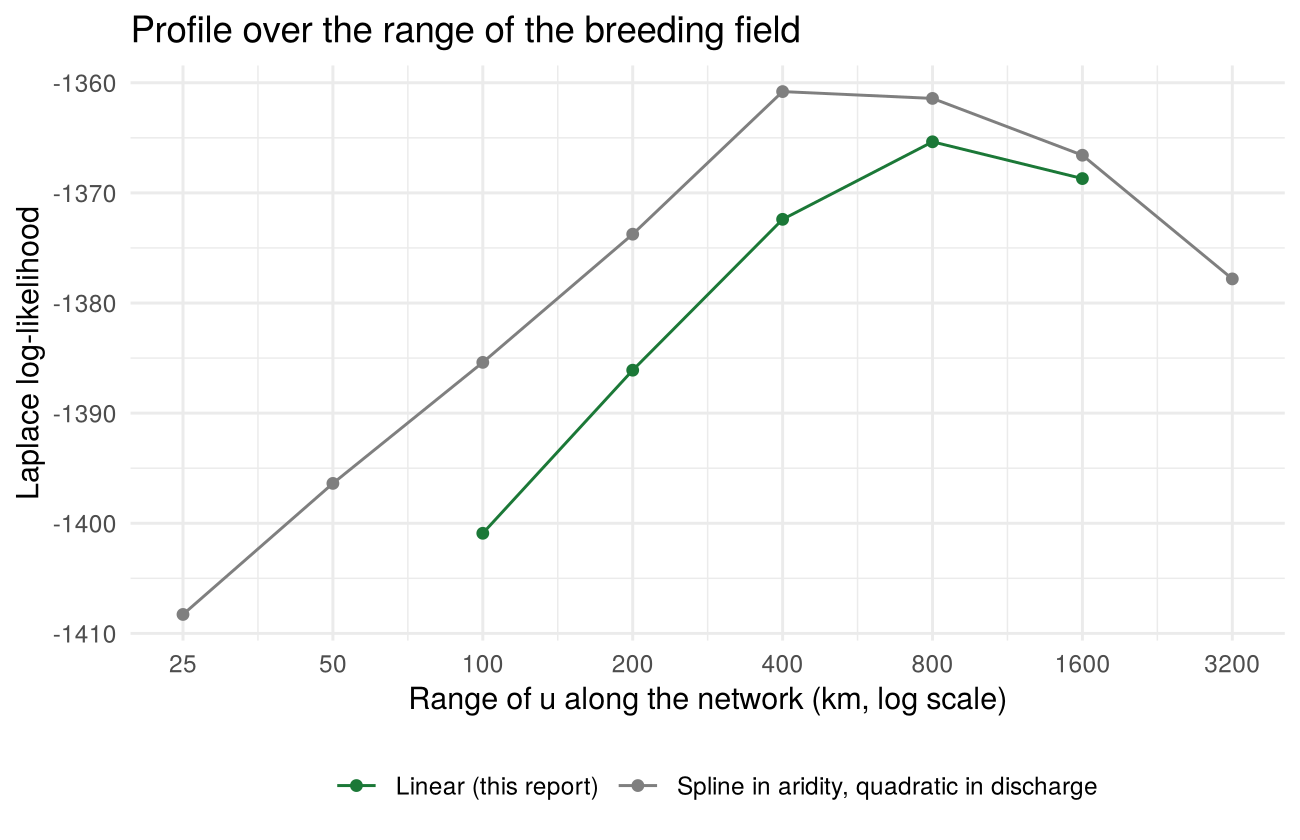
\includegraphics[width=0.7\textwidth]{profile_range_u.png}
\caption{Approximate log-likelihood as a function of the range of the breeding field, for the linear model of this report and for the model with a spline in log aridity and a quadratic in log discharge.}
\label{fig:profile}
\end{figure}

Table~\ref{tab:estimates} reports the regression coefficients. With the breeding field in the model, the effect of aridity is monotone and positive, $\beta_1 = 1.41$ (0.28): doubling the aridity index multiplies the force of infection by $2^{1.41} \approx 2.7$. The effect of discharge is negative, $\theta = -0.29$ (0.11), so that a tenfold increase in discharge roughly halves the breeding intensity per kilometre of river, consistent with small, fast-flowing streams being the main breeding habitat. The standard errors are two to five times larger than without latent effects, because they now account for the residual variation along the rivers and between villages.

\begin{table}[H]
\centering
\caption{Estimates (standard errors) of the linear model. Maximum likelihood without latent effects; posterior mode and Gauss--Newton standard errors, conditional on the variance parameters, with the latent effects.}
\label{tab:estimates}
\begin{tabular}{lrrr}
\toprule
 & No latent effects & Village effect only & $u$ (800 km) + village effect \\
\midrule
Intercept $\beta_0$ & $-3.33$ (0.20) & $-3.34$ (0.19) & $-3.12$ (0.37) \\
$\log \AI$, $\beta_1$ & 1.47 (0.05) & 1.20 (0.13) & 1.41 (0.28) \\
$\log Q$, $\theta$ & $-0.94$ (0.13) & $-0.23$ (0.12) & $-0.29$ (0.11) \\
$\sigma_u$ & -- & -- & 2.76 \\
$\sigma_Z$ & -- & 2.21 & 0.89 \\
\bottomrule
\end{tabular}
\end{table}

Figure~\ref{fig:u} shows the mode of $u$ on the rivers within reach of a village. The largest values are on the Nile between Abu Hamad and the confluence with the Atbara, the stretch where the river crosses the Fourth and Fifth Cataracts and where the only infected desert villages are found, while the slow stretches of the Nile further north and south and the White Nile have negative values. In South Sudan the field is positive over the dense networks of small streams in the west and centre and in the far south-east. The field therefore identifies the river features that discharge cannot describe, and this is what allows the effects of discharge and aridity to be linear: in the earlier model without $u$, the Abu Hamad focus produced the change point in the aridity effect, with a negative slope in the driest conditions, and the increase in breeding for the largest rivers.

\begin{figure}[H]
\centering
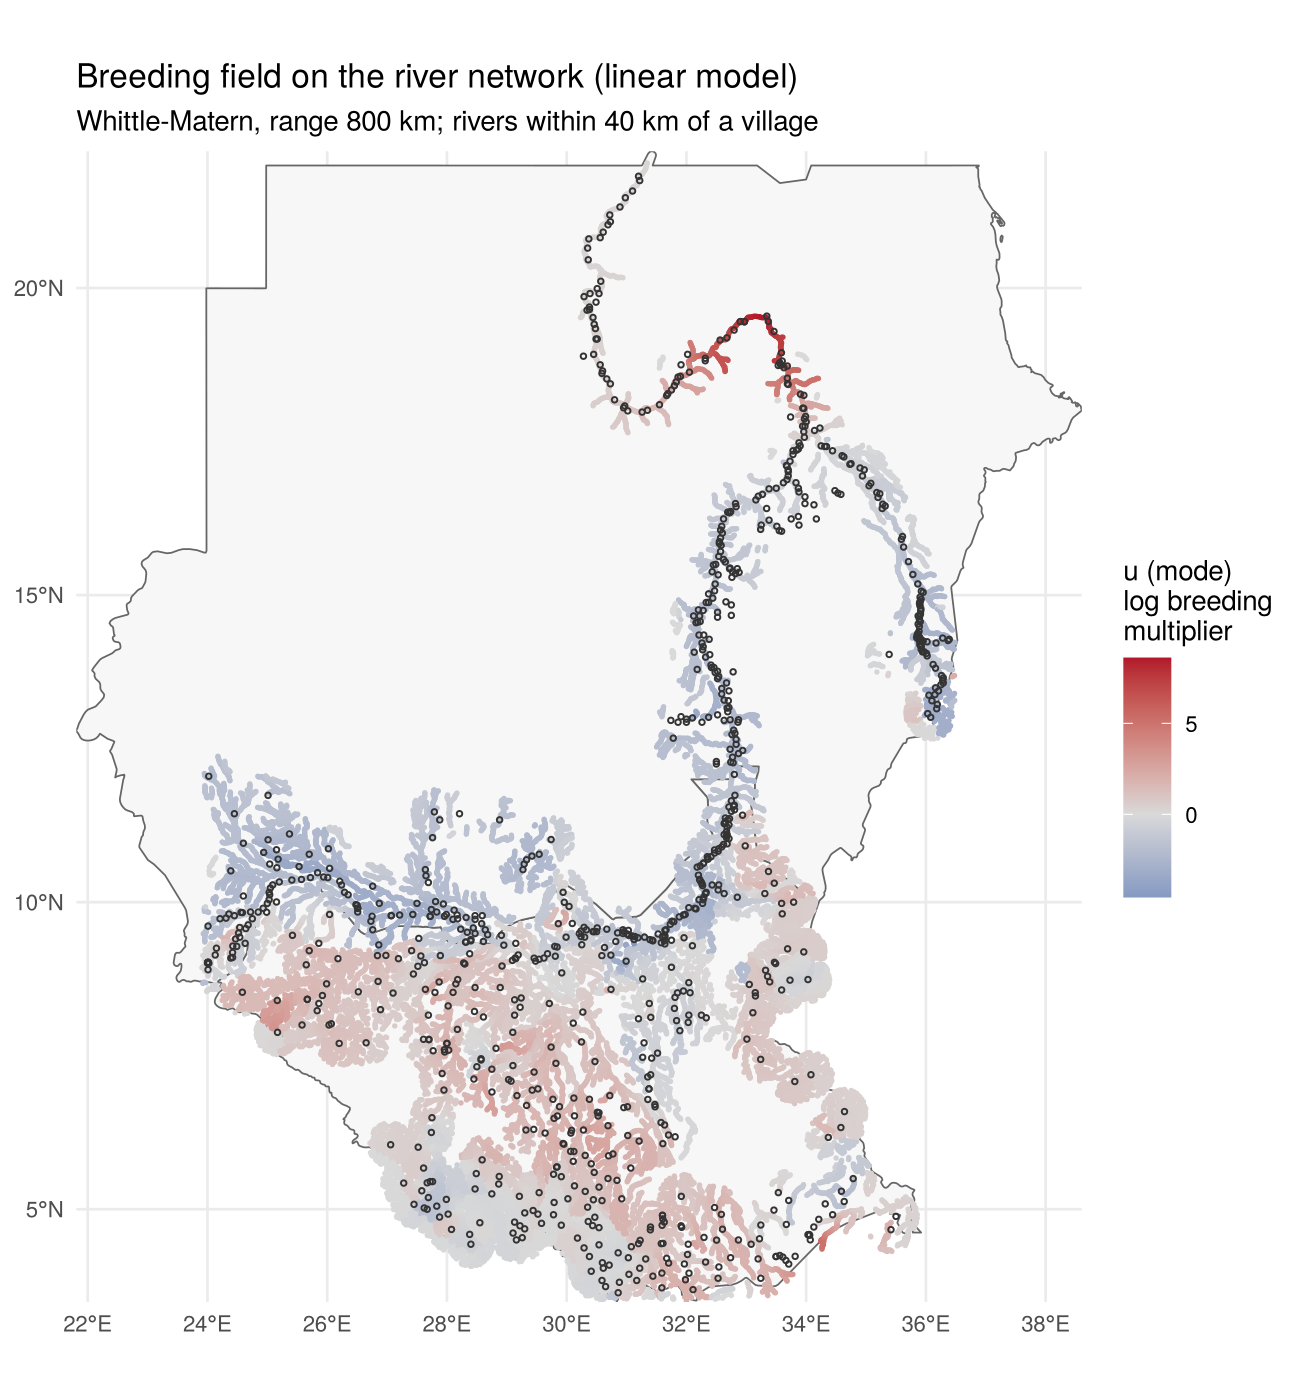
\includegraphics[width=0.49\textwidth]{u_field_map_linear.png}\hfill
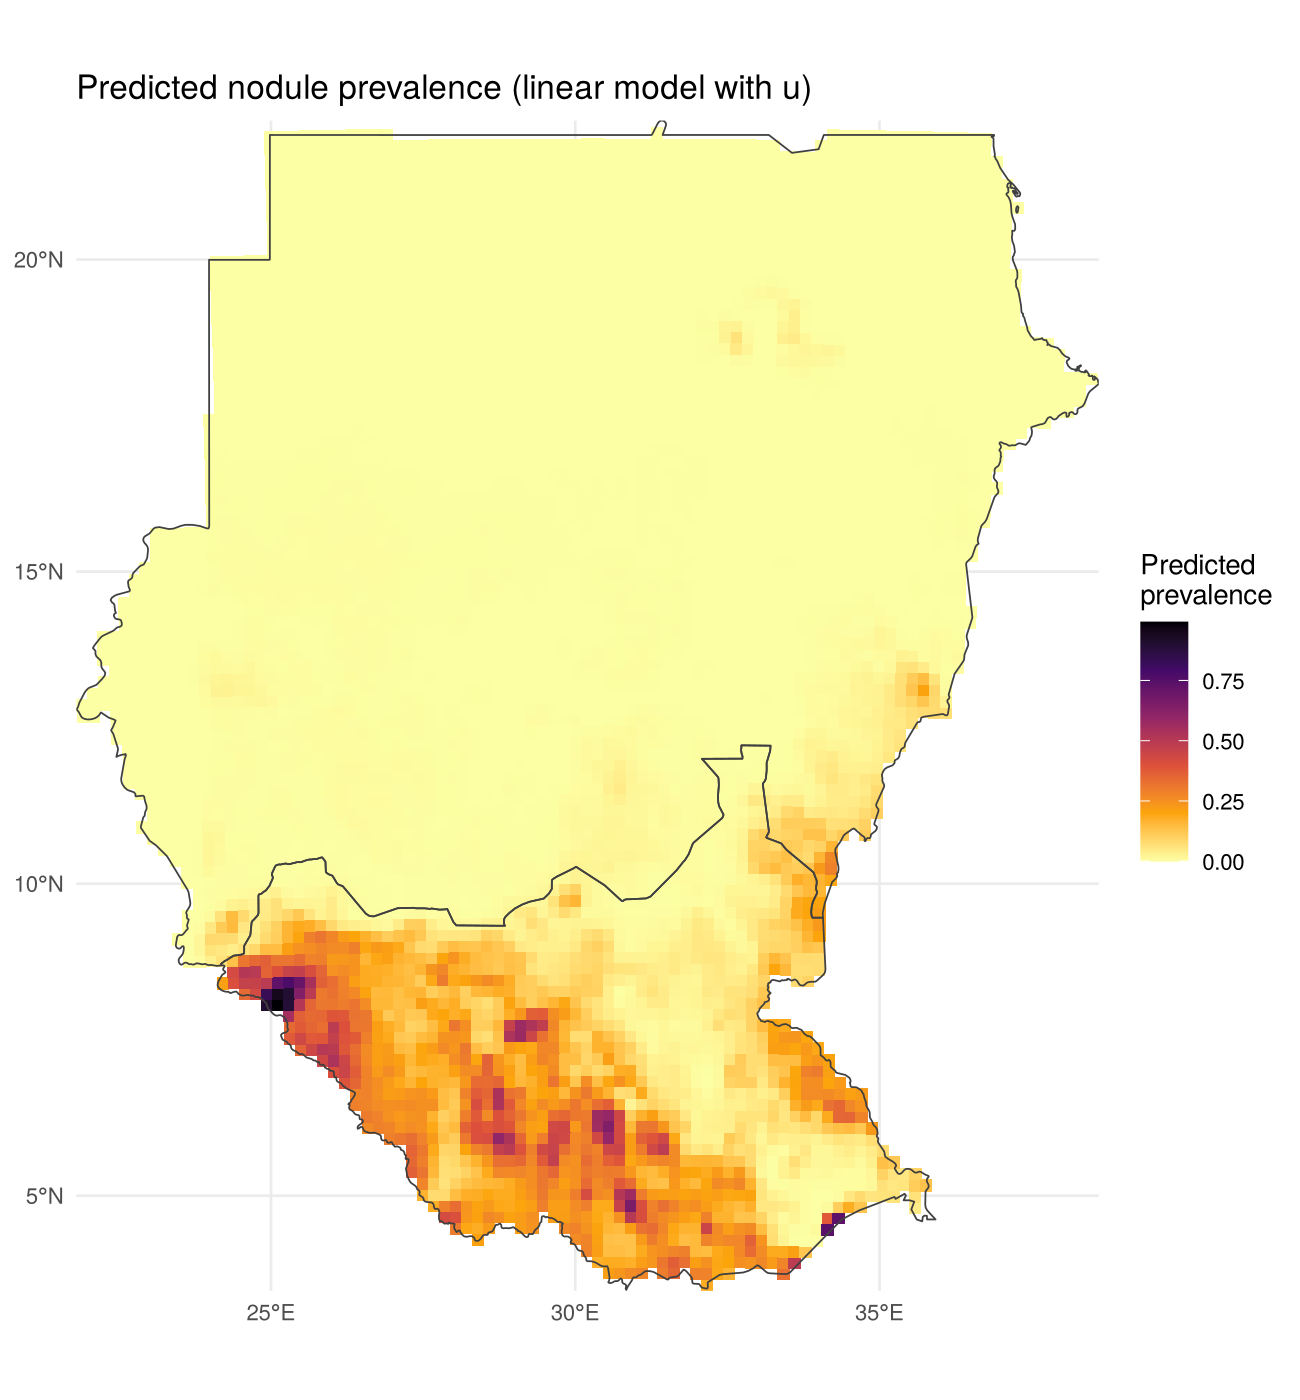
\includegraphics[width=0.49\textwidth]{pred_prevalence_u_linear.png}
\caption{Left: mode of the breeding field $u$ (log multiplier of the breeding intensity) on the rivers within 40~km of a village; circles are the villages. Right: predicted prevalence on a 20~km grid, at the mode of $u$ and with the village effect set to zero.}
\label{fig:u}
\end{figure}

The predicted prevalence (Figure~\ref{fig:u}, right) is close to zero across the desert and the Sahel, except along the Nile near Abu Hamad, and is highest in the south-west and centre of South Sudan and in the far south-east. Observed and predicted prevalence at the villages have a correlation of 0.88, against 0.58 for the linear model without latent effects (Figure~\ref{fig:obs}), and the prevalence by aridity class is reproduced closely (Table~\ref{tab:classes}). These are in-sample comparisons in which $u$ has been estimated from the same villages, so they overstate predictive performance; cross-validation is needed for an honest assessment. The predictions underestimate the highest prevalences, because they are evaluated at the mode with the village effect set to zero, which gives the median rather than the mean force of infection.

\begin{figure}[H]
\centering
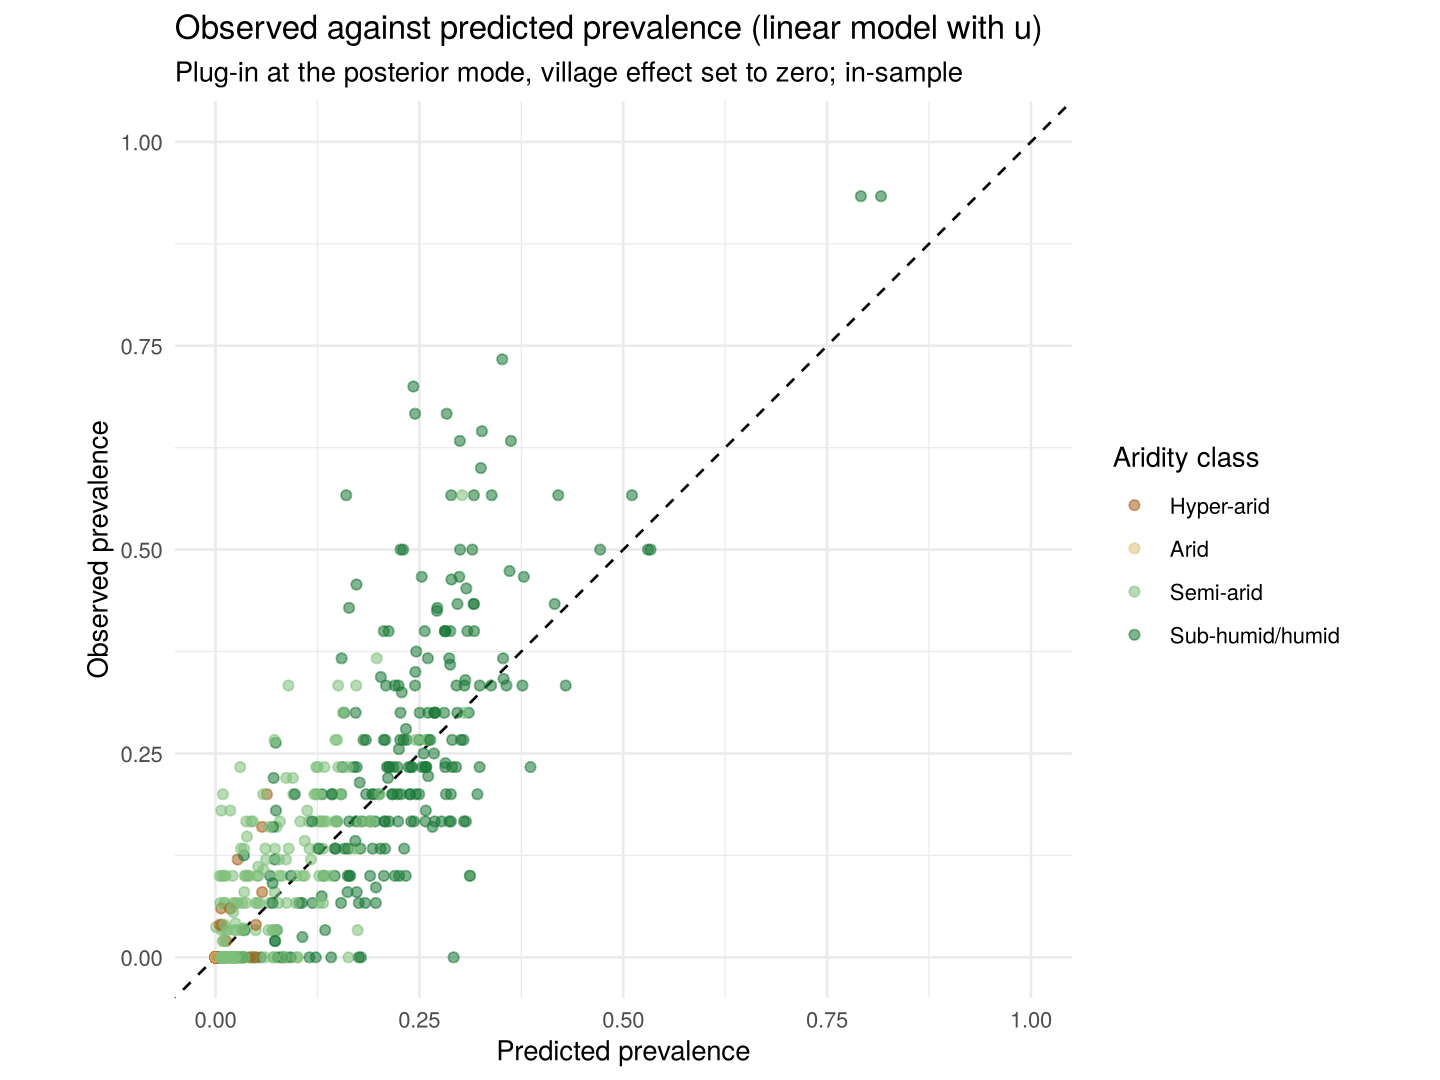
\includegraphics[width=0.7\textwidth]{obs_vs_pred_u_linear.png}
\caption{Observed against predicted prevalence at the 900 villages for the linear model with the breeding field (in-sample).}
\label{fig:obs}
\end{figure}

\begin{table}[H]
\centering
\caption{Observed and predicted prevalence by aridity class (totals of positives over totals examined).}
\label{tab:classes}
\begin{tabular}{lrrr}
\toprule
Aridity class & Observed & Predicted, no latent effects & Predicted, with $u$ \\
\midrule
Hyper-arid ($\AI < 0.05$) & 0.005 & 0.001 & 0.003 \\
Arid (0.05--0.20) & 0.000 & 0.005 & 0.000 \\
Semi-arid (0.20--0.50) & 0.033 & 0.055 & 0.028 \\
Sub-humid and humid ($\AI > 0.50$) & 0.252 & 0.197 & 0.228 \\
\bottomrule
\end{tabular}
\end{table}

\section{Comparison with the more flexible specification and discussion}

The same model with a spline in log aridity and a quadratic in log discharge reaches an approximate log-likelihood of $-1360.80$, at a range of 400~km, against $-1365.36$ for the linear model, a difference of 4.6 units for two additional coefficients and an estimated change point. Since the regression coefficients are integrated out, these marginal likelihoods include a penalty for each coefficient that depends on its prior standard deviation, so the comparison is indicative; but both specifications describe the data similarly once the breeding field is included. In the flexible specification with $u$, the slope of the aridity effect below the change point is $-0.8$ with a standard error of about 0.5 and the quadratic term in discharge is not significant, so its additional features are no longer supported. We therefore prefer the linear model, which has a monotone effect of aridity with a clear interpretation, a single parameter for the effect of river size, and attributes the remaining variation to the rivers and to the villages.

The decomposition of the force of infection into exposure and intensity of transmission is retained and sharpened. The exposure now depends on the rivers through both their discharge and the field $u$, which acts as a map of the suitability of the river network for breeding, and the intensity of transmission through aridity and a village effect. Places beyond 40~km of any river still have zero exposure. Several points need attention. First, $u$ is informed only on the rivers within reach of a village, so elsewhere its mode is close to zero and its uncertainty large; predictions in unsurveyed basins inherit this uncertainty, which the plug-in maps do not show. Second, the range of $u$ is large and its variance at the ends of the network is twice that in the interior, as implied by the Kirchhoff conditions; a field with smoothness $\alpha = 2$ or a stationary boundary correction could be considered. Third, the field may be partly explained by measured river characteristics, such as channel gradient and the seasonality of flow from RiverATLAS, which would turn part of $u$ into interpretable covariates. Finally, predictive performance should be assessed by cross-validation, and uncertainty in predictions obtained by sampling from the Laplace approximation.


\begin{thebibliography}{9}

\bibitem[Bolin et al.(2024)]{bolin2024}
Bolin, D., Simas, A.~B. and Wallin, J. (2024).
\newblock Gaussian Whittle--Mat\'ern fields on metric graphs.
\newblock \textit{Bernoulli}, 30(2), 1611--1639.

\bibitem[Carnaghi et al.(2024)]{carnaghi2024}
Carnaghi, M. et al. (2024).
\newblock Short- and long-range dispersal by members of the \textit{Simulium damnosum} complex (Diptera: Simuliidae), vectors of onchocerciasis: a review.
\newblock \textit{Insects}, 15(8), 606.

\bibitem[Lehner and Grill(2013)]{lehner2013}
Lehner, B. and Grill, G. (2013).
\newblock Global river hydrography and network routing: baseline data and new approaches to study the world's large river systems.
\newblock \textit{Hydrological Processes}, 27, 2171--2186.

\bibitem[Steihaug(1983)]{steihaug1983}
Steihaug, T. (1983).
\newblock The conjugate gradient method and trust regions in large scale optimization.
\newblock \textit{SIAM Journal on Numerical Analysis}, 20(3), 626--637.

\bibitem[Wendland(1995)]{wendland1995}
Wendland, H. (1995).
\newblock Piecewise polynomial, positive definite and compactly supported radial functions of minimal degree.
\newblock \textit{Advances in Computational Mathematics}, 4, 389--396.

\bibitem[Zomer et al.(2022)]{zomer2022}
Zomer, R.~J., Xu, J. and Trabucco, A. (2022).
\newblock Version 3 of the Global Aridity Index and Potential Evapotranspiration Database.
\newblock \textit{Scientific Data}, 9, 409.

\end{thebibliography}

\end{document}
